% -------------------------------------------------------
%  Section 9: Porting to the embedded domain
% -------------------------------------------------------
\section{انتقال به دامنه نهفته: مجموعه‌داده \lr{ARM/Zephyr}}
\label{sec:arm}

\subsection{انگیزه}
پرسش دوم \S\ref{sec:critique}، یعنی انتقال‌پذیری ایده به دامنه‌ای غیر از \lr{PE}، هدف فاز چهارم بود و با موضوع درس نیز هم‌راستاست. استدلال معنایی مقاله درباره بخش‌ها ویژه ویندوز است: نقش کلیدی \kd{.rsrc} از این فرض می‌آید که گونه‌های یک خانواده آیکون و منوی مشترک دارند، و در سفت‌افزار یک سامانه نهفته چنین بخشی وجود ندارد. پرسش این است که آیا قطعه‌بندی بخش‌محور در نبود این نشانه‌ها هم سودمند می‌ماند.

\subsection{مجموعه‌داده}
مجموعه‌داده از سفت‌افزار‌های ساخته‌شده با سیستم‌عامل بی‌درنگ \lr{Zephyr} \cite{zephyr2024} برای هسته‌های \lr{ARM Cortex-M} تشکیل شده است. ساختار تولید آن چنین است: \num{۵۳۱} برنامه نمونه \lr{Zephyr} روی \num{۲۷۱} بورد هدف ساخته شده‌اند و \num{۱٬۶۰۱} ساخت سالم به دست آمده است. برای هر ردهٔ بدافزار، یک «دستور تزریق» تعریف می‌شود که در آن \emph{دقیقاً یک} فایل منبع از درخت \lr{Zephyr} با یک گونه تغییریافته جایگزین و پروژه از نو ساخته می‌شود. هر رده میان ۱۱ تا ۱۴ دستور تزریق متمایز دارد. جدول \ref{tab:armclasses} توزیع نهایی را نشان می‌دهد.

\begin{table}[!ht]
    \centering
    \footnotesize
    \caption{توزیع کلاس‌ها در مجموعه‌داده \lr{ARM/Zephyr}}
    \label{tab:armclasses}
    \begin{tabular}{|l|c|c|p{6.4cm}|}
    \hline
    \textbf{کلاس} & \textbf{نمونه} & \textbf{دستور تزریق} & \textbf{الگوی رفتاری هدف} \\ \hline
    \lr{benign}          & \num{۱٬۶۰۱} & --- & ساخت سالم بدون تغییر \\ \hline
    \lr{backdoor\_like}  & \num{۵٬۶۴۳} & ۱۴ & مسیر فرمان پنهان در زیرسامانه پوسته یا شبکه \\ \hline
    \lr{byovd\_like}     & \num{۴٬۴۴۹} & ۱۱ & سوءاستفاده از راه‌انداز مجاز برای دسترسی ممتاز \\ \hline
    \lr{geofencing\_like}& \num{۴٬۶۴۷} & ۱۳ & شرطی‌سازی رفتار بر پایه موقعیت یا شناسه شبکه \\ \hline
    \lr{logic\_bomb\_like}& \num{۵٬۱۸۵} & ۱۲ & فعال‌سازی بار مخرب پس از شرط زمانی یا رویدادی \\ \hline
    \lr{rootkit\_like}   & \num{۶٬۰۴۶} & ۱۴ & پنهان‌سازی از مسیر‌های بازرسی سامانه \\ \hline
    \textbf{مجموع}       & \textbf{۲۷٬۵۷۱} & & \\ \hline
    \end{tabular}
\end{table}

دو ویژگی این مجموعه‌داده باید صریح گفته شود، چون بر تفسیر همه نتایج بعدی اثر می‌گذارند. نخست، مجموعه‌داده \textbf{ترکیبی و تولیدشده} است و نه گردآوری‌شده از بدافزار واقعی؛ کلاس‌ها الگوی رفتاری را شبیه‌سازی می‌کنند و پسوند \kd{\_like} در نام آن‌ها همین را می‌رساند. دوم، تفاوت میان یک نمونه سالم و گونه بدافزاری \emph{هم‌تبار} آن، جایگزینی یک فایل منبع از میان حدود صد واحد ترجمه پیوندخورده است. یعنی سیگنال کلاس یک اختلال کوچک و موضعی درون تصویری است که در بقیه نقاط یکسان می‌ماند، در حالی که تنوع میان نمونه‌ها (۵۳۱ برنامه در ۲۷۱ بورد) بسیار بزرگ است. این ساختار، مسئله را از انتساب خانواده در \lr{BIG 2015} به‌مراتب دشوارتر می‌کند و در \S\ref{sec:reassess} به پیامد‌های آن بازمی‌گردیم.

\subsection{نگاشت بخش‌ها از \lr{PE} به \lr{ELF}}
معادل‌های مستقیم \kd{.text}، \kd{.rodata} و \kd{.data} به‌سادگی نگاشت می‌شوند، اما \kd{.rsrc} معادلی ندارد. در عوض، سفت‌افزار \lr{Zephyr} چند بخش ویژه دارد که اطلاعات ساختاری ارزشمندی حمل می‌کنند و ما آن‌ها را به تقسیم‌بندی افزودیم: \kd{rom\_start} که جدول بردار وقفه \lr{Cortex-M} را نگه می‌دارد، \kd{initlevel} که ترتیب مقداردهی اولیه زیرسامانه‌ها را کدگذاری می‌کند، و چهار بخش \kd{device\_area}، \kd{device\_api\_area}، \kd{device\_states} و \kd{sw\_isr\_table} که در مجموع گراف راه‌انداز‌های دستگاه و جدول روال‌های خدمت وقفه را توصیف می‌کنند. این انتخاب انگیزه امنیتی روشنی دارد: رده \lr{byovd\_like} بر سوءاستفاده از راه‌انداز مجاز استوار است، پس جدول‌های راه‌انداز محتمل‌ترین جایی هستند که اثر آن دیده شود.

برای هر نمونه، ۲۱ آرایه ذخیره می‌شود: سه بازنمایی خام \lr{S1}، \lr{S2} و \lr{S3}، و برای هر یک از نُه بخش هدف، یک زیرتصویر \lr{S4} و یک زیرتصویر \lr{S5}. شکل \ref{fig:schemes} این بازنمایی‌ها را برای یک ساخت سالم و گونه \lr{backdoor\_like} هم‌تبار آن نشان می‌دهد.

\begin{figure}[!ht]
    \centering
    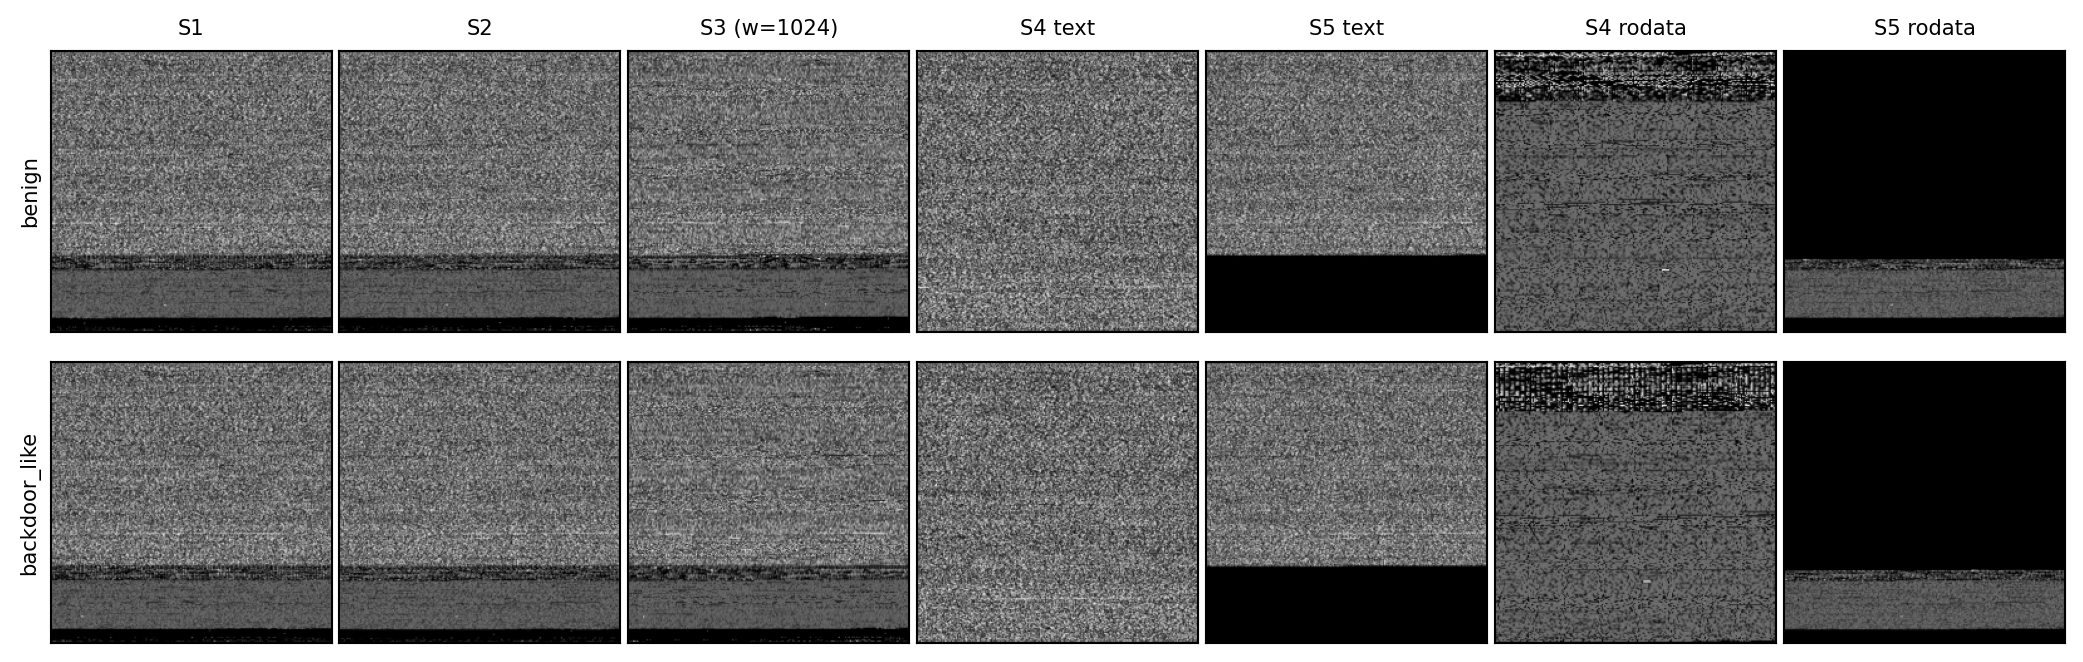
\includegraphics[width=0.95\textwidth]{figs/schemes.png}
    \caption{بازنمایی‌های \lr{S1} تا \lr{S5} برای یک ساخت سالم \lr{Zephyr} (ردیف بالا) و گونه \lr{backdoor\_like} ساخته‌شده از همان ساخت (ردیف پایین). تفاوت دو ردیف با چشم عملاً تمیزناپذیر است، که دشواری مسئله را نشان می‌دهد. تُنُکی شدید \lr{S5} نیز در دو ستون آخر پیداست.}
    \label{fig:schemes}
\end{figure}

\subsection{پروتکل ارزیابی}
برخلاف \lr{BIG 2015}، در اینجا سرور ارزیابی بیرونی با برچسب پنهان وجود ندارد. بنابراین یک تفکیک ۸۰ به ۲۰ لایه‌ای\pn{Stratified} با بذر ثابت \num{۴۲} تعریف کردیم و همه اعداد صحت، \lr{F1} کلان و ضریب همبستگی متیوز\pn{Matthews Correlation Coefficient (MCC)} \cite{chicco2020mcc} که در این گزارش می‌آیند، روی همان \pct{۲۰} نگه‌داشته‌شده محاسبه شده‌اند.

\subsection{نتایج انتقال پایه}
نخستین چرخه آزمایش، انتقال مستقیم روش با همان ابرپارامتر‌های جدول \ref{tab:hyper} و ۲۰ دوره آموزش بود: ۱۹ پیکربندی با توصیف داده \kd{arm\_zephyr} در حالت شش‌کلاسه، بدون هیچ تغییری در رویه آموزش. جدول \ref{tab:armbase} نتیجه را نشان می‌دهد.

\begin{table}[!ht]
    \centering
    \scriptsize
    \caption{انتقال پایه روش به \lr{ARM/Zephyr}؛ ۱۹ پیکربندی، ۲۰ دوره، ابرپارامتر‌های مقاله. سه ستون نخست روی \pct{۲۰} نگه‌داشته‌شده محاسبه شده‌اند.}
    \label{tab:armbase}
    \begin{tabular}{|l|l|c|c|c|c|}
    \hline
    \textbf{مدل} & \textbf{پیکربندی} & \textbf{صحت} & \textbf{\lr{F1} کلان} & \textbf{\lr{MCC}} & \textbf{صحت کل داده} \\ \hline
    \lr{ResNet50} & \lr{S3} & \pct{۶۵٫۷۵} & \num{۰٫۵۶۸۴} & \num{۰٫۵۸۵۶} & \pct{۷۳٫۳۸} \\ \hline
     & \lr{S5: raw + rodata data} & \pct{۶۵٫۲۲} & \num{۰٫۵۶۴۰} & \num{۰٫۵۷۷۵} & \pct{۷۲٫۱۷} \\ \hline
     & \lr{S5: raw + text rodata data (4ch)} & \pct{۶۲٫۲۷} & \num{۰٫۵۴۰۲} & \num{۰٫۵۴۰۳} & \pct{۷۱٫۱۳} \\ \hline
     & \lr{S5: raw + text rodata data romstart (5ch)} & \pct{۶۰٫۱۸} & \num{۰٫۵۱۹۱} & \num{۰٫۵۱۱۶} & \pct{۶۸٫۶۰} \\ \hline
     & \lr{S2} & \pct{۳۱٫۸۶} & \num{۰٫۲۷۰۹} & \num{۰٫۱۵۹۵} & \pct{۴۶٫۸۹} \\ \hline
     & \lr{S5: raw + text rodata} & \pct{۳۱٫۶۸} & \num{۰٫۲۳۰۷} & \num{۰٫۱۶۲۵} & \pct{۳۹٫۶۳} \\ \hline
     & \lr{S5: raw + text data} & \pct{۳۱٫۵۱} & \num{۰٫۲۶۹۴} & \num{۰٫۱۵۶۲} & \pct{۴۳٫۸۴} \\ \hline
     & \lr{S1} & \pct{۳۰٫۹۳} & \num{۰٫۲۳۶۸} & \num{۰٫۱۴۶۲} & \pct{۳۶٫۶۴} \\ \hline
     & \lr{S4: text rodata data} & \pct{۲۹٫۰۳} & \num{۰٫۲۳۷۲} & \num{۰٫۱۳۲۹} & \pct{۳۵٫۴۷} \\ \hline
     & \lr{S5: text rodata data} & \pct{۲۸٫۵۸} & \num{۰٫۱۹۷۲} & \num{۰٫۱۲۳۱} & \pct{۳۴٫۵۳} \\ \hline
     & \lr{S4: text rodata data raw (4ch)} & \pct{۲۴٫۳۳} & \num{۰٫۱۸۶۹} & \num{۰٫۰۷۰۸} & \pct{۲۷٫۰۱} \\ \hline
     & \lr{S4: text rodata data romstart (4ch)} & \pct{۲۱٫۹۹} & \num{۰٫۱۵۰۰} & \num{۰٫۰۴۵۱} & \pct{۲۵٫۰۶} \\ \hline
    \lr{VGG16} & \lr{S3} & \pct{۳۸٫۷۳} & \num{۰٫۳۱۰۶} & \num{۰٫۲۴۷۶} & \pct{۶۰٫۵۴} \\ \hline
     & \lr{S2} & \pct{۳۸٫۷۱} & \num{۰٫۳۱۶۷} & \num{۰٫۲۴۵۸} & \pct{۶۵٫۴۳} \\ \hline
     & \lr{S5: text rodata data} & \pct{۳۷٫۸۶} & \num{۰٫۲۹۶۸} & \num{۰٫۲۳۵۰} & \pct{۵۰٫۸۶} \\ \hline
     & \lr{S5: raw + text data} & \pct{۳۷٫۱۹} & \num{۰٫۲۹۲۶} & \num{۰٫۲۲۸۷} & \pct{۵۷٫۲۶} \\ \hline
     & \lr{S5: raw + text rodata} & \pct{۳۵٫۷۲} & \num{۰٫۲۷۳۹} & \num{۰٫۲۱۵۱} & \pct{۵۳٫۵۵} \\ \hline
     & \lr{S4: text rodata data} & \pct{۳۲٫۵۷} & \num{۰٫۲۶۵۰} & \num{۰٫۱۶۹۴} & \pct{۵۲٫۴۱} \\ \hline
     & \lr{S1} & \pct{۳۱٫۲۱} & \num{۰٫۲۷۲۶} & \num{۰٫۱۵۵۲} & \pct{۵۱٫۶۷} \\ \hline
    \end{tabular}
\end{table}

سه مشاهده از این جدول بیرون می‌آید. نخست، فاصله میان بهترین و بدترین پیکربندی بسیار بزرگ است (\pct{۶۵٫۷۵} در برابر \pct{۲۱٫۹۹}) و برخلاف \lr{BIG 2015} که همه پیکربندی‌ها در محدوده باریکی جمع بودند، در اینجا انتخاب بازنمایی تعیین‌کننده است. دوم، \lr{VGG16} در تمام پیکربندی‌ها به‌مراتب ضعیف‌تر از \lr{ResNet50} است؛ با توجه به ایراد «ب» در \S\ref{sec:critique} این مقایسه نیز مخدوش است، چون ابرپارامتر‌های دو مدل متفاوت مانده‌اند. سوم و مهم‌تر از همه، بررسی سنجه‌های درون‌کلاسی بهترین مدل نشان داد که \textbf{بازخوانی کلاس \lr{benign} دقیقاً صفر است}: مدل حتی یک نمونه از \num{۳۲۰} نمونه سالم مجموعه نگه‌داشته‌شده را درست تشخیص نمی‌دهد و همه را به یکی از پنج ردهٔ بدافزار نسبت می‌دهد. این فروپاشی کامل کلاس اقلیت، انگیزه اصلی چرخه بعدی آزمایش‌ها شد.
